\documentclass[10pt,a4paper]{article}
\usepackage[utf8]{inputenc}
\usepackage[spanish]{babel}
\usepackage{amsmath}
\usepackage{amsfonts}
\usepackage{amssymb}
\usepackage{graphicx}
\usepackage{multicol}
\usepackage{titling}
\usepackage{titlesec}
\usepackage{array}
\usepackage{bm}
\usepackage{afterpage}
\usepackage{float}
\usepackage{graphicx}
\usepackage{epstopdf}
\usepackage{longtable}
\usepackage{xcolor}
\usepackage{epigraph}
\setlength\epigraphwidth{1.5\textwidth}
\usepackage{subfigure}
\usepackage{anyfontsize}
\usepackage[left=2cm,right=2cm,top=2cm,bottom=2cm]{geometry}
\usepackage[colorlinks=true,
            linkcolor=blue,
            citecolor=blue,
            urlcolor=blue]{hyperref}

\begin{document}
\author{Lisseth C. Alban-Checa} % CAMBIAR A AUTORES
\title{MATERIA DE SISTEMAS EMBEBIDOS\\ % TITULO  \\ ES ENTER
PROYECTO FINAL - Trabajo Individual Simulado}
\maketitle  
\section{Introducción} % nuevas secciones
\begin{multicols}{2} % texto en 2 colomnas
Los sensores ultrasónicos miden la distancia mediante el uso de ondas ultrasónicas. El cabezal emite una onda ultrasónica y recibe la onda reflejada que retorna desde el objeto. Los sensores ultrasónicos miden la distancia al objeto contando el tiempo entre la emisión y la recepción.\\
\\Un sensor de presión es un instrumento compuesto por un elemento detector de presión con el que se determina la presión real aplicada al sensor (utilizando distintos principios de funcionamiento) y otros componentes que convierten esta información en una señal de salida. \\
\\Despues de tener los conceptos claros de los materiales que vamos a usar para nuetro proyecto simulado, tenemos que aclarar que en eld esarrollo del proyecto tuvimos algunas dificultades, en especial con el modo sleep que nos pide desarrollar debido a que no se puede usar las mismas librerías del Arduino Uno en Arduino Megay es necesario usar el arduino mega para desarrollar el modo sleep ya que las matrices que se necesitan pra esa parte del proyecto sobrepasan la memoria del arduino uno que hemos usado durante este materia en el transcurso de este curso.
\end{multicols} %termina texto en columnas
\section{Diseño del Sistema}
\subsection{Diagrama de Flujo}
Ingresar su diagrama de flujo realizado en cualquier programa.
\begin{figure}[ht!]
\caption{Diagrama de flujo} % ingresa nombre de la figura (caption)
\centering
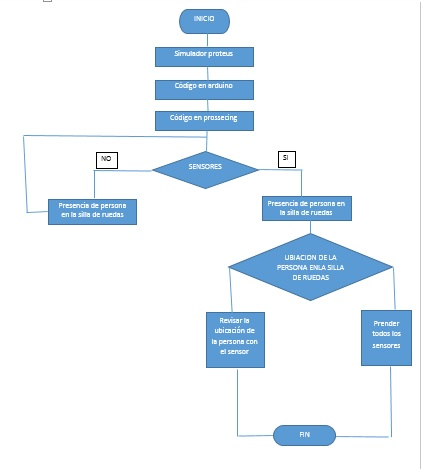
\includegraphics[scale=0.4]{DIAGRAMA DE FLUJO.jpg} % cambie el valor de la escala entre 0.1-1 para el tamano de la misma
\end{figure}\\ %termina figura y envia enter
Ingrese su diagrama de bloques
\begin{figure}[hbt!]
\caption{Diagrama de bloques} % ingresa nombre de la figura (caption)
\centering
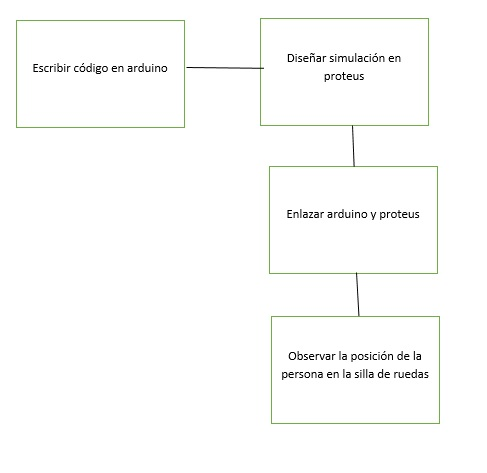
\includegraphics[scale=0.25]{DIAGRAMA DE BLOQUES.jpg}
\end{figure}

\section{Desarrollo}

\subsection{Simulación}
Ingrese su simulación

\begin{figure}[ht!]
\caption{Simulacion en proteus}
\centering
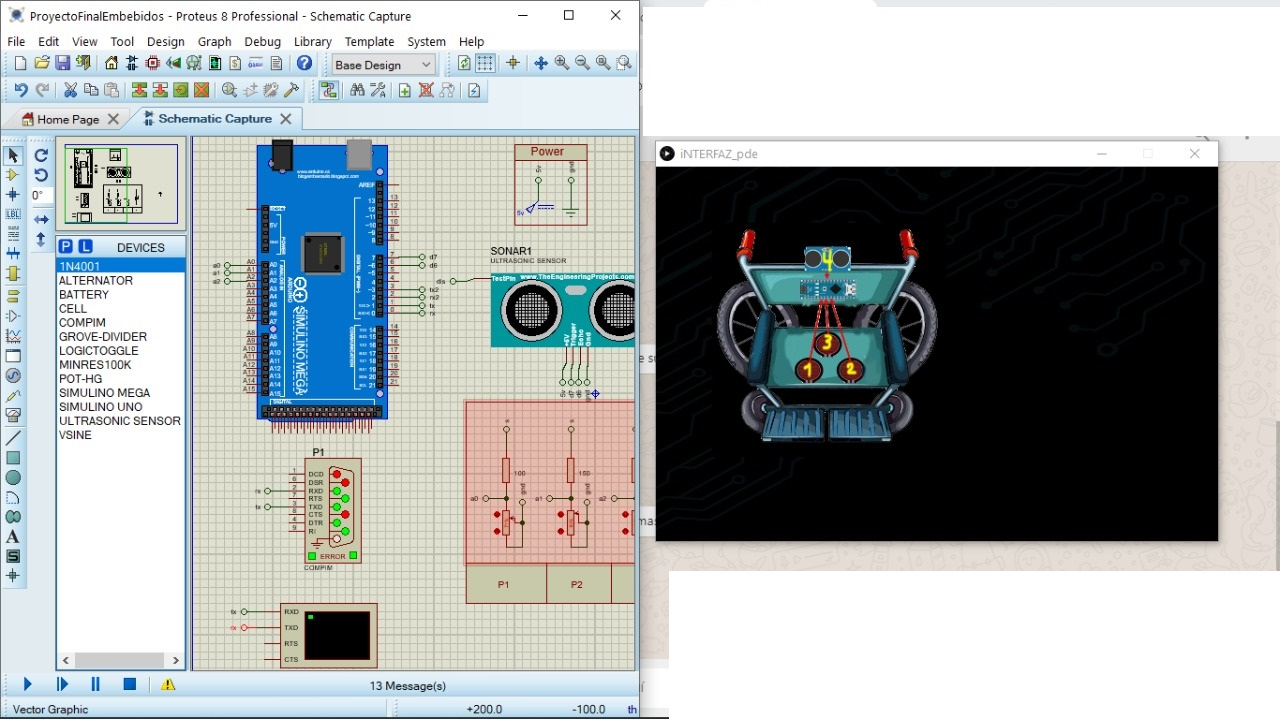
\includegraphics[scale=0.5]{SIMULACION.jpg}
\end{figure} 


\section{Análisis de Resultados}
\begin{figure}[ht!]
\caption{Codigo en arduino}
\centering
\includegraphics[scale=0.5]{CODIGO_AR.jpg}
\end{figure} 
\begin{figure}[ht!]
\caption{Codigo en prossecing}
\centering
\includegraphics[scale=0.5]{CODIGO_PROS.jpg}
\end{figure} 
\begin{figure}[ht!]
\caption{Simulacion en proteus}
\centering
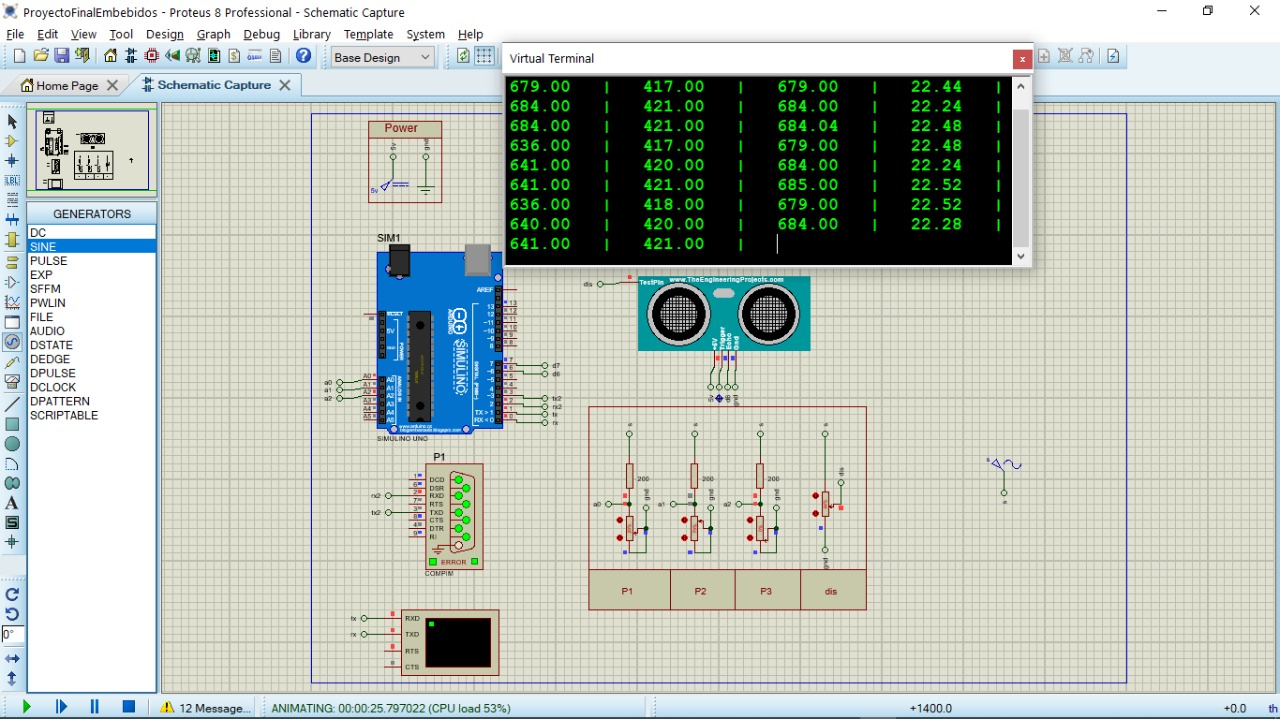
\includegraphics[scale=0.5]{SIMULACION_PRO.jpg}
\end{figure} 

\section{Conclusiones y Recomendaciones}
\subsection{Conclusiones}
\begin{itemize}
\item La utilizacion de las herramientas de diseño es muy util en cuanto al prototipado para el aspeco fisico de los proyectos que se dean realizar.
\item La utilizacion del sistema arduino y la silumacion del programa proteus con la union del programa prossecing es de gran ayuda para el desarrollo de esta materiay de los proyectoa realizarce para el aprendizaje.
\end{itemize}
\\
\subsection{Recomenciones}
\begin{itemize}
\item Revisar que las librerias sean la indicadas para la realizacion de los proyectos a ejecutarse.
\item Saber representar la lógica de programación al sistema de simulación esto hará́ que se facilite los procesos al momento de crear nuestro proyecto.
\end{itemize}
\end{document}